% !TeX document-id = {1952f704-6c22-4b23-a625-e40904df778f}
%%% File encoding: UTF-8
%%% äöüÄÖÜß  <-- keine deutschen Umlaute hier? UTF-faehigen Editor verwenden!

%%% Magic Comments zum Setzen der korrekten Parameter in kompatiblen IDEs
% !TeX encoding = utf8
% !TeX program = pdflatex 
% !TeX spellcheck = de_DE
% !BIB program = biber

\documentclass[master,english,smartquotes]{hgbthesis}
% Zulässige Optionen in [..]: 
%   Typ der Arbeit: diploma, master (default), bachelor, internship
%   Hauptsprache: german (default), english
%		smartquotes: zur vereinfachten Eingabe von Hochkommas (nur "...")
%%%----------------------------------------------------------

\RequirePackage[utf8]{inputenc}		% bei der Verw. von lualatex oder xelatex entfernen!

\graphicspath{{images/}}    % Verzeichnis mit Bildern und Grafiken
\logofile{logo}							% Logo-Datei = images/logo.pdf (\logofile{}, wenn kein Logo gewünscht)
\bibliography{references}  	% Biblatex-Literaturdatei (references.bib)

%%%----------------------------------------------------------
% Angaben für die Titelei (Titelseite, Erklärung etc.)
%%%----------------------------------------------------------

%%% Einträge für ALLE Arbeiten: -----------------------------
\title{Analysis of Unreachable Code using Static Code Analysis}
\author{Lukas Braun, BSc}

%\programtype{Fachhochschul-Bachelorstudiengang}		% select/edit
\programtype{Fachhochschul-Masterstudiengang}

\programname{Software Engineering}
\placeofstudy{Hagenberg}
\dateofsubmission{2021}{08}{31}	% {YYYY}{MM}{DD}

\advisor{Dipl.-Ing. (FH) Dr. Josef Pichler}	% optional

%\strictlicense		%%% restrictive license instead of Creative Commons (discouraged!)

%%%----------------------------------------------------------
\begin{document}
%%%----------------------------------------------------------

%%%----------------------------------------------------------
\frontmatter                    % Titelei (röm. Seitenzahlen)
%%%----------------------------------------------------------

% \maketitle
\tableofcontents

% \chapter{Preface}
\label{cha:Preface}
 				% Vorwort ist optional
\chapter{Abstract}
\label{cha:abstract}


% This thesis is about the detection of unreachable code in source code. %This type of error occurs in two forms, either due to unconditional jumps using imperative statements, which is easily detected, or due to infeasible conditions, which is harder to detect, since a broader context is needed to determine feasibility.
% Unreachable code has two different causes, on the one hand it is caused by unconditional jumps by imperative statements, which is easily detected, on the other hand due to infeasible conditions, since a broader context is needed to determine feasibility.

% Unreachable code is not only checked by specific static code analysis tools,  but also provided as a check by the compiler or an integrated development environment. Many solutions for different programming languages exist, but do not check unreachable code to the same extent. For example, compilers usually do not even determine unreachable code, others are designed to not even compile when unreachable code is encountered (e.g., javac).


% In this thesis this check was introduced to an existing static code analysis, which targets structured text, a pascal-like language included in the IEC-61131-3 standard. This analysis requires to represent the program in form of a control flow graph and simplifies passing every path. The context contains possible values for every variable in form of predicates. These predicates may be checked for feasibility by an SMT-solver, which is able to determine possible concrete values for each variable. 

% At this point, the implemented approach only works on small, constructed examples. However, the implementation is able to find special cases of unreachable code that no other tool examined was able to find. Since not all language features were taken into account (e.g. arrays, structures) the implementation is not complete and should therefore rather be considered as incomplete.

% Funktioniert auf kleinen Beispielen, manche Sprach features nicht berücksichtigt (Strukturen, Arrays, etc.)
% Funktioniert auf nicht zu komplexen Beispielen (Loops bringen probleme mit sich --> Laufzeit)
% Eher als Prototyp zu betrachten, wird aber in Zukunft weiter geführt werden.

This paper is about the detection of unreachable code in source code. 
Unreachable code has two different causes, on the one hand by unconditional jumps and on the other hand by unfeasible conditions.

Unreachable code is not only checked by specific static code analysis tools, but also provided as a check by the compiler or an integrated development environment. There are many solutions for different programming languages, but they do not check unreachable code to the same extent. For example, compilers usually do not detect unreachable code, while others are designed to provide a translation error when unreachable code occurs.


In this thesis, detection of unreachable code was built into an existing static code analysis targeting Structured Text, a Pascal-like language included in the IEC-61131-3 standard. This analysis requires the representation of the program to be analyzed in the form of a control flow graph, because this graphical representation transfers sequences without jumps into nodes, while jumps are represented in the form of edges. Possible values are carried along for each variable in the form of constraints. These constraints can be translated into a language that an SMT solver checks for satisfiability. 

At this point, the implemented approach only works on small, constructed examples. For this, the implementation is able to find special cases of unreachable code that no other tool studied was able to find. Since not all language features were taken into account (e.g. arrays, structures) the implementation is not complete and should therefore rather be considered as incomplete.


\chapter{Kurzfassung}

\begin{german}
In dieser Arbeit geht es um die Erkennung von unerreichbarem Code im Quellcode. Diese Art von Fehlern tritt in zwei Formen auf, entweder aufgrund von unbedingten Sprüngen mit Hilfe von imperativen Anweisungen, was leicht zu erkennen ist, oder aufgrund von undurchführbaren Bedingungen, was schwieriger zu erkennen ist, da ein breiterer Kontext erforderlich ist, um die Durchführbarkeit zu bestimmen.


Unerreichbarer Code wird nicht nur durch spezielle statische Code-Analyse-Tools überprüft, sondern auch durch den Compiler oder eine integrierte Entwicklungsumgebung. Es gibt viele Lösungen für verschiedene Programmiersprachen, die jedoch nicht in gleichem Maße auf unerreichbaren Code prüfen. So stellen Compiler normalerweise nicht einmal unerreichbaren Code fest, andere sind so konzipiert, dass sie nicht einmal kompilieren, wenn unerreichbarer Code auftritt (z. B. javac).


In dieser Arbeit wurde diese Prüfung in eine bestehende statische Codeanalyse eingeführt, die auf strukturierten Text abzielt, eine Pascal-ähnliche Sprache, die in der Norm IEC-61131-3 enthalten ist. Diese Analyse erfordert die Darstellung des Programms in Form eines Kontrollflussgraphen und vereinfacht das Durchlaufen jedes Pfades. Der Kontext enthält mögliche Werte für jede Variable in Form von Prädikaten. Diese Prädikate können von einem SMT-Solver auf Machbarkeit geprüft werden, der in der Lage ist, mögliche konkrete Werte für jede Variable zu bestimmen. 

\end{german}

%%%----------------------------------------------------------
\mainmatter          % Hauptteil (ab hier arab. Seitenzahlen)
%%%----------------------------------------------------------

\chapter{Introduction}
\label{cha:introduction}

% \chapter {State of the Art}
\label {cha:state of the art}

\chapter {Theoretical Foundation}
\label {cha:theoretical foundation}

%!TEX root = ../main.tex

\chapter{State of the Art}
\label{cha:state of the art}

Analyzing code is a central part of software development. Naturally, this process can be automated to some degree using various static code analysis tools. 
Some of these tools are applied at different stages during development ranging from compilation time to static code analysis in the cloud. 
Generally, static code analysis benefits by detecting errors and problematic constructs early, but also highlights code that does not adhere to coding guidelines.


In this chapter multiple static code analysis tools will be presented, ranging in quality for detecting bugs (with a focus on unreachable code).
The accuracy for finding unreachable code increases with each tool presented. 
The examples are provided in form of Java source code beginning with the Java compiler (OpenJDK \cite{OpenJDK} implementation) itself, which verifies the correctness of source code before code generation. 


One of the most important tools a programmer uses is the Integrated Development Environment (IDE), which is capable of additional code inspection and highlighting errors and warnings. 
The most popular Java IDEs are Eclipse \cite{incCommunityOpenInnovation} and IntelliJ \cite{IntelliJIDEACapable}. 
Possibly both may be improved by installing additional plugins for checking code.


Sonarqube \cite{sonarqube} is a static code analysis tool hosted in the cloud and usually is part of a continuous integration pipeline. It offers a wide variety of checks including a more in-depth unreachable code analysis.


Some instances of unreachable code may not be found using the tools mentioned before. For a more advanced approach statements have to be evaluated. Infeasible path conditions, described in Section \ref{sub:infeasible code}, may be found by using a mathematical prover or SMT-Solver.
\clearpage
\pagebreak
\section{Java Compiler}
\label{sec:Java compiler}
% Javac also used by IDEs. 

The Java compiler (OpenJDK \cite{OpenJDK}) performs checks regarding unreachable code that strictly result in a compile time error. 
In the official documentation \cite{Chapter14Blocks} unreachable code is defined as follows:
\begin{quote}
This section is devoted to a precise explanation of the word "reachable." 
The idea is that there must be some possible execution path from the beginning of the constructor, method, instance initializer, or static initializer that contains the statement to the statement itself. The analysis takes into account the structure of statements. Except for the special treatment of while, do, and for statements whose condition expression has the constant value true, the values of expressions are not taken into account in the flow analysis.
\label{quote:Java unreachable definition}
\end{quote}

Since values are not considered during this analysis, it is impossible to detect infeasible code as described in Listing \ref{code:Java infeasible undetected}.
 Loops are the exception here, but only conditions containing literal boolean values will be checked and may result in a compile time error as demonstrated by Listing \ref{code:Java loop unreachable}. The rationale behind not considering the values of variables and even constants is to use them to switch on and off source code fragments (see Listing \ref{code:Java flags}).


Unexpected return statements turn the following statements unreachable. As shown in Listing \ref{code:Java unexpected return} and mentioned before, conditions of if-then-else blocks are not evaluated, even if they contain only (boolean) literals. 


Unexpected break statements turn the following statements within the current scope of the loop unreachable as shown in Listing \ref{code:Java unexpected break}.


\begin{program}[h!]
	\begin{JavaCode}
void testUnreachableWhile() {
	int x = 3;
	while(false || false && true) x = 10; // Compile time error
}

void testUnreachableWhileNoError() {
	int x = 3;
	while(false || false && true || x == 4) x = 10; // No error
}

void testUnreachableWhileBoolean() {
	int x = 3;
	boolean y = false;
	while(false || false && true || y) x = 10; // No error
}\end{JavaCode}
	\caption{The Java compiler evaluates conditions of loops, if, and only if, they contain literal boolean values only.}
	\label{code:Java loop unreachable}
\end{program}

\begin{program}[h!]
	\begin{JavaCode}
void testSimpleIf() {
	int x = 3;
	if(false) x = 10; // No error
}\end{JavaCode}
	\caption{Simple if-then-else statements do not evaluate the condition at all.}
	\label{code:Java infeasible undetected}
\end{program}

\begin{program}[h!]
	\begin{JavaCode}
void testFlag() {
	int x = 3;
	final boolean DEBUG = false;
	if(DEBUG) x = 10; // No error
}\end{JavaCode}
	\caption{The rationale behind not even considering constant values is the usage of flags.}
	\label{code:Java flags}
\end{program}

\begin{program}[h!]
	\begin{JavaCode}
void testSystemExit() {
	System.exit(0);
	int x = 0; // no error - System.exit is not handled like a return statement
}

void testAlwaysReturn() {
	if(true) return;
	int x = 0; // no error - condition is not checked
}

void testReturn() {
	return;
	int i = 3; // Compilation error - unreachable statement
}

void testReturnInAllBranches() {
	boolean x = true;
	if(x) return;
	else return;
	x = false; // Compilation error - unreachable statement
}

void testReturnInWhile() {
	while(true) {
		return;
	}
	int i = 34; // Compilation error - unreachable statement
}\end{JavaCode}
	\caption{Examples of unreachable code due to unexpected return statements. Interestingly System.exit(), a statement that does terminate the program, is not handled like a return statement.}
	\label{code:Java unexpected return}
\end{program}

\begin{program}[h!]
	\begin{JavaCode}
void testBreak() {
	while(true) {
		int i = 3;
		break; 
		i++; // Compilation error - unreachable statement
	}
}

void testBreak2() {
	while(true) {
		int i = 3;
		if(true) break; 
		i++; // no error - condition is not checked
	}
}\end{JavaCode}
	\caption{Examples of unreachable code due to unexpected break statements.}
	\label{code:Java unexpected break}
\end{program}
%% TODO Liveness beschreiben
% Regarding unreachable code the Java compiler performs a data-flow analysis. The liveness of each statement will be analyzed. The implemented AST-model makes use of the visitor pattern \cite{gammaDesignPatternsElements}. 


\clearpage
\pagebreak
\section{Integrated Development Environments}
\label{sec:intelliJ}
Integrated Development Environments (IDE) are used by almost every software developer daily and are an integral tool for creating and refactoring code.
In comparison to simple text editors IDEs extend text editors with tools that make it one the on side easier to write code (e.g., by providing snippets that can be inserted, autocomplete) and by providing some sort of static code analysis to assist a developer while writing code.
Depending on the IDE, static code analysis can be configured to be more or less strict. 
When the IDE contains an extensive plugin system, then custom-made analysis tools may be used for even more precise method to find potential bugs.


Regarding unreachable code the following IDEs were analyzed:
\begin{itemize}
	\item \emph{Eclipse} \cite{incCommunityOpenInnovation} is an IDE primarily focused on developing Java projects. The IDE provides its own compiler \cite{teamJDTCoreComponent}, which does not only compile projects, but is also responsible for static code analysis. Additional to the checks by the OpenJDK \cite{OpenJDK} Java compiler, conditions in if-then-else expressions are also evaluated and checked by default. When values of variables are known, then they will be considered in the analysis as shown in Listing \ref{code:Java eclipse intelij always true or false}. Generally, the eclipse Java compiler is very basic regarding unreachable code detection. As shown in Listing \ref{code:Java eclipse fail to find this} its compiler does not even consider the same condition in an if/else-if block. Other datatypes (e.g., int) are also taken into account. Besides that Eclipse is extensible and many additional tools for more sophisticated analysis exist.
	\item \emph{IntelliJ Idea} \cite{IntelliJIDEACapable} is an IDE used for developing projects in various popular programming languages (e.g., Java, C\#, Python, JavaScript). For the Java language, a code inspector can be configured to find different categories of errors. By default two important rules are activated to deliver warnings: 
	\begin{itemize}
		\item \emph{Constant conditional expressions}, which do not only check for boolean literals in conditions, but also take values of variables, in case they always have the same value, and even other data types (e.g., int) into account as shown in Listing \ref{code:Java eclipse intelij always true or false}
		\item \emph{Duplicate condition} that have already been checked. Even though this may sometimes be intended, in most cases they are overlooked or may even not be reached, when the method terminates in the branch followed by the former condition as shown in Listing \ref{code:Java intelij duplicate conditions}. 
	\end{itemize}
	IntelliJ also provides a plugin system and therefore the possibility integrating an even better analysis is given.
\end{itemize}

% Beispiele für eclipse + IntelliJ

\begin{program}[h!]
	\begin{JavaCode}
void testAlwaysTrueCondition() {
	if(true) return; // Warning: Condition is always true
	int i = 3;
}

void testAlwaysFalse() {
	boolean x = true;
	boolean y = false;
	if(x && y) int i = 3; // Warning: Condition is always false
}

void testUnreachableWhile() {
	int x = 3;
	while(x > 4) x = 10; // Warning: Condition is always false
}\end{JavaCode}
	\caption{Internal code inspection tools of the IDEs \emph{Eclipse} and \emph{IntelliJ Idea} are capable of detecting conditions, which always evaluate to true or false.}
	\label{code:Java eclipse intelij always true or false}
\end{program}

\begin{program}[h!]
	\begin{JavaCode}
void testCondAlreadyChecked(boolean x) {
	int y = 0;
	if(x) {
		y = 3;
	} else if(x) { // Condition already checked before
		y = 4;
	}
	y++;
}\end{JavaCode}
\caption{Eclipse does not even check for duplicate conditions within the same if/else-if block. In contrast IntelliJ does find this issue.}
\label{code:Java eclipse fail to find this}
\end{program}

\begin{program}[h!]
	\begin{JavaCode}
void duplicateConditions(int s_operationHour, int m_operationHour) {
	if(s_operationHour != m_operationHour) { // Warning: Duplicate condition
		m_operationHour = s_operationHour;
		if (s_operationHour == 0) {
			foo();        
		}
		return;
	}
	if(s_operationHour == 0) {
		m_operationHour = 0;
	} else {
		// Unreachable, since the condition was checked already and returned
		if(s_operationHour != m_operationHour) { // Warning: Duplicate condition
			s_operationHour = m_operationHour;
		}
	}
}\end{JavaCode}
	\caption{Even though these warnings do not hint to the unreachable code directly. Duplicate condition in different branches of an if statement show a code smell prone to errors. In this particular case the else branch of the second if-then-else block cannot be reached, since the method already returned. Removing the return statement in line 7 removes this type of problem, but the second condition would always evaluate to false. }
	\label{code:Java intelij duplicate conditions}
\end{program}
\newpage
\section{Sonarqube and Sonarlint} 
\label{sec:sonar}
\emph{Sonarqube} \cite{sonarqube} and \emph{Sonarlint} \cite{SonarLintFixIssues} are products created by \emph{Sonarsource} \cite{CodeQualityCode}. Sonarqube is a static code analysis solution used in conjunction with a build server.
Commonly this analysis is either triggered after pushing commits, scheduled at certain times of the day or a combination of both.
Sonarqube supports a multitude of programming languages like Java, C\#, Python, COBOL and more. Another language may be supported in form of a plugin.


Sonarlint is available for some IDEs (including Eclipse and IntelliJ) in form of a plugin to provide immediate feedback. Note that this plugin only covers a subset of functionalities of sonarqube, but still provides better support than many internal inspectors built into IDEs.

\newpage
% Mutations beschreiben
Using the same example as before (seen in Listing \ref{code:Java intelij duplicate conditions}) Sonarqube detects that this expression always evaluates to false, which provides better information than the internal code inspector of IntelliJ, as demonstrated in Listing \ref{code:Java sonarqube duplicate conditions}. The example shown in Listing \ref{code:Java sonarqube hard example} cannot be detected. It appears that reassignments in loops are not evaluated and therefore no error is delivered. This type of error may only be detected by evaluating each statement.


\begin{program}[h!]
	\begin{JavaCode}
void duplicateConditions(int s_operationHour, int m_operationHour) {
	if(s_operationHour != m_operationHour) {
		m_operationHour = s_operationHour;
		if (s_operationHour == 0) {
			foo();        
		}
		return;
	}
	if(s_operationHour == 0) {
		m_operationHour = 0;
	} else {
		if(s_operationHour != m_operationHour) { // SonarLint: Change this Condition so it does not always evaluate false
			s_operationHour = m_operationHour;
		}
	}
}\end{JavaCode}
	\caption{The same example as seen in Listing \ref{code:Java intelij duplicate conditions}, but sonarqube reports the problem correctly. }
	\label{code:Java sonarqube duplicate conditions}
\end{program}

\begin{program}[h!]
	\begin{JavaCode}
void testLoop(boolean pred) {
	int x = 1;
	do {
		boolean b = x != 1;
		// b can never be true, this will possibly result in an infinite loop.
		if(b) {
			pred = false;
		}
	} while(pred);
}

void testDeadCode() {
	int i, j;
	i = 3;
	for(j = 1; j < i; ++j) {
		// ...
	}
	// i must be equal to j
	if(i != j) { 
		// ...
	}
}\end{JavaCode}
	\caption{Neither the internal code inspector of IntelliJ nor Eclipse nor sonarlint/-qube were able to catch these errors. }
	\label{code:Java sonarqube hard example}
\end{program}

\clearpage
\section{Joogie}
\label{sec:sca paper}
Joogie \cite{arltJoogieInfeasibleCode2012, arltJoogieJavaJimple2013} identifies infeasible code of any Java-project using a verification system. 
At first the source code will be transformed into a 3-address intermediate representation of Java bytecode using the Soot \cite{Soot} framework. 

Afterwards the Java bytecode is transformed into the Boogie language \cite{BoogieIntermediateVerification}, which is an imperative intermediate verification language for analyzing high-level programming languages.
During the translation the memory model has to be preserved. The heap is represented by a two-dimensional array. The first index refers to the object's address and the second to the field of the object.

Loops are unwound into three unwindings: the first and last iteration, as well as an abstract unwinding of the rest.
The result is a program containing no loops. Every assignment inside the loop replaces the value into non-determined values. Therefore loops are not fully evaluated.


Methods are checked in an intraprocedural manner. Therefore variables that may change become non-deterministic. 


Afterwards the Boogie program will be called by the verifier. 
The foundation of the verifier is the SMT-solver Z3.



When infeasible code is encountered, the java bytecode will be transformed back into Java and a violation will be reported.


This tool was tested on 4 bigger open source software projects including ArgoUML \cite{ArgoUMLResourcesSite}, Rachota \cite{RachotaTimetracker} and Freemind \cite{MainPageFreeMind}, and only few false warnings were reported.
The time needed for analysis was tolerable, since usually only small code fragments have to be analyzed instead of the whole project.

Since this is an older project relying on a special version of Z3 \cite{demouraZ3EfficientSMT2008}, which is not available anymore, it could not be tested in the course of this thesis. Neither of these two research papers \cite{arltJoogieInfeasibleCode2012, arltJoogieJavaJimple2013} do provide concrete examples, which instances of unreachable and infeasible code can be found.

% This tool is probably as capable as Sonarqube \cite{sonarqube} in finding unreachable code.


%!TEX root = ../main.tex

\chapter{Finding Unreachable Code Using an SMT-Solver}
\label{cha:finding unreachable code using a smt-solver}

The developed approach uses the control flow graph as a basis, but does not transform it into single static assignment form.
During analysis the control flow graph will be traversed and interpreted until every possible execution path was followed and analyzed.
After each interpretation state (e.g., assignments, path conditions) will be added accordingly and must be taken into account.
Merging state has to be handled correctly to make correct statements about the current value of a variable.
The state is represented in the form of a predicate, which may be checked by a system capable of determining satisfiability (e.g., an SMT-solver).
Satisfiable results will continue with the next block(s) and using the new state as a basis and flag this block as visitable.
Unsatisfiable results stop the computation at the current block and will not pursue to continue the path.
Therefore this method is pessimistic.
By using this method, every error should be found in theory (as described in Chapter \ref{cha:conclusion}), since every instruction will be handled like during execution. 
This entails barriers such as 
\begin{itemize}
	\item Significant increase in time needed for analysis. 
	\item Possibly exponentially growing expressions to determine satisfiability.
\end{itemize}
These problems lead to greater execution time, which requires the implementation of reactions (e.g., early stopping, assuming values for variables in loops).

\section{Architecture}
The implementation is part of an already developed static code analysis tool \cite{Prahofer_2012}. 
It consists of different parsers, forms of representation and a rule executor. 
As shown in Figure \ref{fig:general architecture} the tool requires IEC source code and a configuration file for the rule executor.
Basically, rules are Java classes which check if the given IEC source code does not violate any conventions or contain bad code smells. 
Some rules collect metrics, such as lines of code, code complexity, nesting level, cohesion and coupling.
Rules get triggered by certain nodes of the abstract syntax tree, like declarations of variables, function calls, arithmetic expression, et cetera.
For analysis the rule executor traverses the abstract syntax tree and triggers the specified rules provided in the configuration file.
Rules may need different representations of these nodes for more sophisticated analysis. 
When rules are not met, violations will be generated. They contain position, causation and the error message. Violations are written to an XML file, which can be imported to Sonarqube\cite{sonarqube}.


The detection of unreachable code will be implemented in form of a rule as seen in Figure \ref{fig:unreachable-architecture-overview}, the next Section \ref{sec:translation} covers the translation from the abstract syntax tree to a general control flow graph. 
Afterwards the instructions within the control flow graph will be transformed as described in Section \ref{subsec:translate instructions}.
The analysis is covered in Section \ref{sec:analysis}.

\begin{figure}
	\centering
	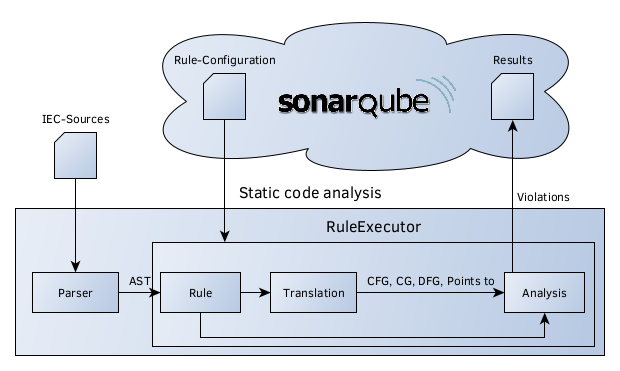
\includegraphics[width=1\textwidth]{static-code-analysis}
	\caption{Architectural overview of the static code analysis tool for IEC source code. After parsing IEC source code, the AST will be passed to the RuleExecutor, which triggers only the configured rules. For more advanced analysis, the AST may be transformed into a different representation. When the source code does not conform to the rules violations will be generated, which can be integrated with Sonarqube.}
	\label{fig:general architecture}
\end{figure}

\begin{figure}
	\centering
	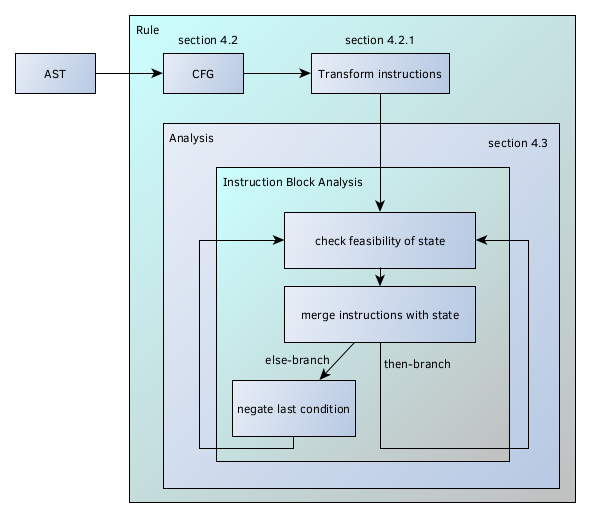
\includegraphics[width=1\textwidth]{unreachable-architecture-overview}
	\caption{General overview of the implementation of the unreachable code detection rule. Each step is annotated in which section it is described. }
	\label{fig:unreachable-architecture-overview}
\end{figure}

\section{Translation of Functions}
\label{sec:translation}
For every function the control flow graph will be calculated and used as the basis. 
Consider the concrete example show in Figure \ref{code:transformation example} as input. 
After parsing the abstract syntax tree will be generated and then used to build the control flow graph (demonstrated in Figure \ref{fig:ast to cfg}).
Information about parameters and global-/system variables also need to be provided in order to handle function-/procedure calls. 
Two separate procedures will be performed on this control flow graph.
\begin{enumerate}
	\item \emph{Unreachable code due to unconditional jumps} is easy to find after the control flow graph was created. Every block (except the beginning block) which does not have any incoming edges must be unreachable.
	Note that these types of errors may also be found as described in Section \ref{sec:analysis}, but were filtered out before.
	\item \emph{Unreachable code due to infeasible conditions} needs a sophisticated and more expensive (in terms of computing resources) approach to identify. The following Section \ref{sec:analysis} describes how to detect them.
\end{enumerate}

\begin{program}
	\begin{GenericCode}
$x$ $\leftarrow$ 3
$y$ $\leftarrow$ 0
		
if $x$ > 2 then
	$y$ $\leftarrow$ $x$ + 1
else
	$y$ $\leftarrow$ $x$ - 1
end
		
while $y$ < $x$ + 10 do
	$y$ $\leftarrow$ $y$ + 1
end
		
log($\downarrow$ $x$)\end{GenericCode}
	\caption{Example containing assignments, branches, loops and procedure-calls. }
	\label{code:transformation example}
\end{program}

\begin{figure}
	\centering
	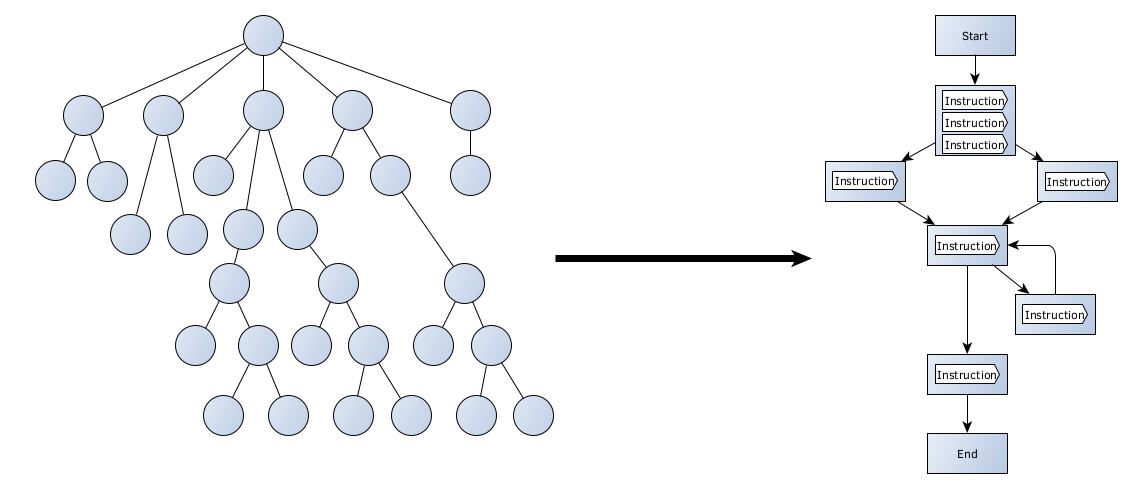
\includegraphics[width=1\textwidth]{ast-to-cfg}
	\caption{In the first step, the abstract syntax tree of a function in listing \ref{code:transformation example} will be translated into the control flow graph.}
	\label{fig:ast to cfg}
\end{figure}


\subsection{Translation of Instructions}
\label{subsec:translate instructions}
The structure of the control flow graph is only one of the necessary components. 
Simplifying instructions makes the overall analysis easier, since each type must be handled differently.
The internal structure of instructions will also be simplified into an AST like structure (see Figure \ref{fig:cfg to internal}). 
Note that the previous control flow graph also contained instructions, which simply were references to nodes in the original AST. 
The new representation contains only the necessary information, which was decoupled from the original AST.

Instructions come in three different types (shown in Figure \ref{fig:state}) and must be marked accordingly:
\begin{enumerate}
	\item \emph{Assignments} are usually the most common form of instructions. They denote a change of the underlying value of a variable and therefore update the state (of said variable) during analysis. 
	\item \emph{Conditions} occur only as the last instruction of a block from a \emph{Controlflow graph}. Note that the last instruction does not necessarily have to be a \emph{condition}.
	\item \emph{Procedure calls} may be mutable and could change variables if they are applied as \emph{output parameters}. % Procedure calls will be dissolved into \emph{assignments} during analysis.
	For intraprocedural analysis of procedures, output parameters will be dissolved into assignments to simplify the process. Basically, it is assumed that out parameters get an undetermined value assigned, which consequently update the state of the variable and may contain any possible value (restricted only by the datatype).
\end{enumerate}
\begin{figure}
	\centering
	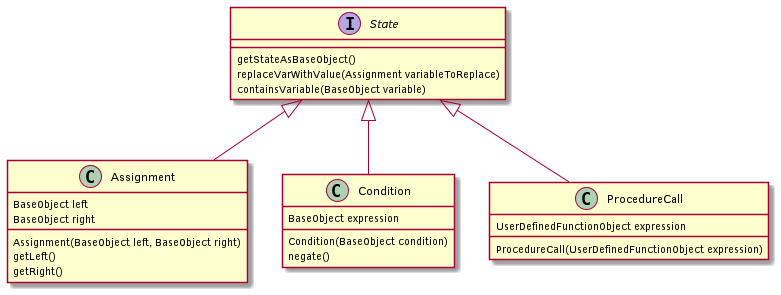
\includegraphics[width=0.85\textwidth]{State}
	\caption{Each instruction in any program may be either represented as an \emph{Assignment}, \emph{Condition} or \emph{ProcedureCall} which encapsulates the expression of types described in Figure \ref{fig:smtobject}. Instructions are processed into a \emph{BaseObject} during evaluation. \emph{Conditions} and \emph{ProcedureCalls} simply contain the expression, whereas \emph{Assignments} separate the left side (the receiving variable) and its concrete value on the right side.}
	\label{fig:state}
\end{figure}
\begin{figure}
	\centering
	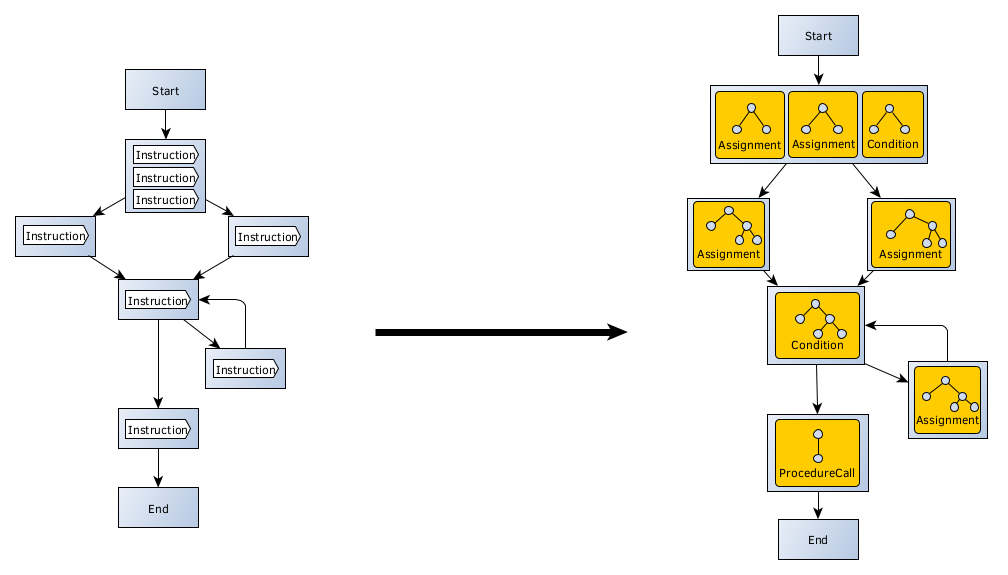
\includegraphics[width=1\textwidth]{cfg-to-internal}
	\caption{The instructions contained in the control flow graph (created before as described in Figure \ref{fig:ast to cfg}) change their representation into a simpler form. As demonstrated in Figure \ref{fig:state} all instructions are either assignments, conditions or procedure calls. Furthermore the concrete instructions are also represented simpler as described in Figure \ref{fig:smtobject}. }
	\label{fig:cfg to internal}
\end{figure}

% AST-Object representation of instructions
Every instruction will also be represented in an AST-like notation as shown in Figure \ref{fig:smtobject}. Each symbol, for example a variable, name of a function or any given literal (such as numbers and strings), are represented as a \emph{BaseObject}. Functions are, in fact, just a special form of this \emph{BaseObject}, which may contain variables. Functions are not only direct function-/procedure calls, but also operations (like + and -). User-defined functions will also be represented as a special form of the described \emph{FunctionObject} before, which contain the declaration of parameters (since named parameters are a language feature of IEC and therefore must be handled correctly), which will be represented as \emph{BaseObjects}. 
This kind of representation makes it easy to work with, since it is a very easy, tree-like data structure which may be traversed easily. Not only replacing variables and values may be done effortlessly, but also the generation of \emph{SMT-Lib} code, since this representation is similar to \emph{LISP}.

\begin{figure}
	\centering
	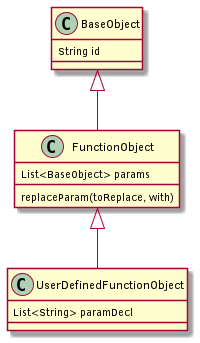
\includegraphics[width=0.2\textwidth]{SMTObject}
	\caption{\emph{AST}-like representation of instructions. }
	\label{fig:smtobject}
\end{figure}
\section{Analysis}
\label{sec:analysis}
After the translation of all functions and instructions the analysis begins. As mentioned in the introduction of this chapter the control flow graph of every function (and procedure) will be traversed. The analysis begins at the single begin block of the graph and ends when all feasible paths reached the exit block. Instruction blocks will be evaluated in order - the same as a program would execute them. 
For each instruction block the instructions will be evaluated. The resulting state must be carried along the analysis and merged correctly to assure valid results. At the end of an instruction block an SMT-solver is used to determine if the current state is feasible or not. Infeasible state may be reached by a combination of conditions. If the current state is infeasible, the \emph{next} block must be unreachable, since the condition at the end of an instruction block determines which branch the flow follows. 
For the determination, if the current state is feasible or not, the SMT-solver Z3 \cite{demouraZ3EfficientSMT2008} is used. The state will be simply translated into the universal, standardized, LISP-like SMT-Lib language \ref{code:translation} which most of the common SMT-solvers are able to interpret. 
If an instruction block is reachable (at least on one occasion), it will be marked as reachable. At the end of the analysis all remaining instruction blocks are marked unreachable.

\begin{program}
	\begin{GenericCode}
procedure $mergeState$($\downarrow$ $instruction$, $\updownarrow$ $state$) begin
	if $instruction.isCondition()$ then
		$state.add($$\downarrow$ $instruction$$)$
	else if $instruction.isAssignment()$ then
		// replace all occurences of variables with their concrete values
		// from the provided $states$ variable
		$replaceVariables($$\updownarrow$ $instruction$, $\downarrow$ $state$$)$ 
		// remove old state e.g. former Assignments and Conditions, which are not
		// valid anymore
		$removeAllOccurrences($$\updownarrow$ $state$, $\downarrow$ $instruction$$)$
		// add the new instruction to the state
		$state.add($$\downarrow$ $instruction$$)$
	end 
end	\end{GenericCode}
	\caption{Merges the new instruction into the existing state. While conditions simply may be added, assignments alter the state, since the concrete value changes and former state can no longer be associated with this variable. }
\label{code:merge state}
\end{program}
\begin{program}
	\begin{GenericCode}
function $solve$($\downarrow$ $state$) begin
	// translate state to SMT-String and pass to Z3
	return $Z3.solve($$\downarrow$ $state.toSMTString())$
end\end{GenericCode}
	\caption{The form (see figure \ref{fig:smtobject}) all instructions are represented in makes the generation of SMTLib code easy. The string containing SMTLib code will simply be passed to the solver directly.}
\label{code:z3 solver}
\end{program}
\begin{program}
	\begin{GenericCode}
procedure $resolveFunctionCalls$($\downarrow$ $instruction$, $\updownarrow$ $state$) begin
	// intra-procedural aprroach:
	// simply remove all variables, which may change.
	$outParams$ $\leftarrow$ $instructions.getOutParams()$
	$state.removeState($$\downarrow$ $outParams$$)$
end	\end{GenericCode}
	\caption{Function calls will be handled in an intra-procedural manner. This is simply realized by just removing any state containing a variable which may change and will be handled like an assignment, whereas the new value is unknown. }
	\label{code:intraprocedural analysis}
\end{program}
\begin{program}
	\begin{GenericCode}
procedure $analyze$ ($\downarrow$ $instructionBlock$, $\downarrow$ $oldState$) begin
	$newState$ $\leftarrow$ $oldState$
	$instructions$ $\leftarrow$ $instructionBlock.getInstructions()$
	$feasible$ $\leftarrow$ $solve(\downarrow oldState)$
		
	if $feasible$ then
		// This instruction block is marked as visitable
		$markInstructionBlock(\downarrow instructionBlock)$ 
		for $instruction$ in $instructions$ do
			$resolveFunctionCalls$($\downarrow$ $instruction$, $\updownarrow$ $newState$)	
			if not $instruction.containsFunctionCall()$ then
				// Functioncalls were already handled at this point
				$mergeState$($\downarrow$ $instruction$, $\updownarrow$ $newState$)
			end 
		end
		$analyze$($\downarrow$ $instructionBlock.getThenBranch()$, $\downarrow$ $newState$)
		// By following the else-branches last instruction, if it was a condition, must be negated
		$analyze$($\downarrow$ $instructionBlock.getElseBranch()$,$\downarrow$ $newState.negateLastInstruction()$)
	end
end	\end{GenericCode}

	\caption{The main component of the unreachable code detection is the analysis of instruction blocks. Beginning with no state set it will be added subsequently by traversing the control flow graph and adding accumulated state. 
	At first the current state must be checked for feasibility. Only if it is feasible (see Listing \ref{code:z3 solver}) this the instruction block can be marked as reachable and new instructions may be added to the state as described in Listing \ref{code:merge state} and Listing \ref{code:intraprocedural analysis}.	
	Afterwards the possible branches will be followed (a maximum of two) containing the new assembled state.}
	\label{code:instruction block analyzer}
\end{program}

% TODO: add example for translation
\begin{program}
	\begin{GenericCode}
$i$ $\leftarrow$ 1
$x$ $\leftarrow$ 5
if $i$ < $x$ then 
	// ...
end\end{GenericCode}
	\begin{GenericCode}
;; Check if condition evaluates TRUE
(declare-fun x () Real)
(declare-fun i () Real)
(assert (and (= i 1) (= x 5) (< i x)))
(check-sat)
; => SAT\end{GenericCode}
	\begin{GenericCode}
;; Check if condition evaluates FALSE	
(declare-fun x () Real)
(declare-fun i () Real)
(assert (and (= i 1) (= x 5) (not (< i x))))
(check-sat)
; => UNSAT\end{GenericCode}
	\caption{Translation of the IEC-Code. As shown above, each variable must be declared beforehand (therefore the implementation must be aware of the type). The assertion includes the complete state (including assignments and conditions). Conditions are the only part which could lead to an unfeasible result. Every Instruction-Block must contain at least one edge out of the block (with the exception of the exit block), but may also contain a second edge, indicating the path of a condition evaluates false. Therefore the condition must be negated.}
	\label{code:translation}
\end{program}

\subsection{Interpretation of Instructions}
\label{sub:Interpretation of Instructions}
% Handling of and state management
One of the central parts during analysis is the handling of states. Each instruction must have the same effect as it was executed after compilation. 
As described before, states come in three forms: assignment, condition, procedure-/function call, which all must be handled accordingly (see the implementation in Listings \ref{code:intraprocedural analysis} and \ref{code:merge state}): 

\begin{itemize}
	\item Conditions are just added to the state as they are. 
	\item Assignments have to be handled differently. Assignments change the current value of a variable and therefore the path condition is not valid afterwards. It must be reset therefore. 
		If there is any variable on the right side, it must be replaced by its value. Especially cases which contain the same variable on the left and right side must use the values instead of the identifier, since a SMT solver does not contain any mechanism for reassignment, but rather a bidirectional unification. For example the statement (= x (+ x 1)) will always result in an unsatisfiable state.
	\item Procedure-/function-calls will be handled as described in \ref{sub:handling procedure and function calls}. Out parameters and the return values are represented as assignments. 
\end{itemize}

After all instructions are interpreted, it will be translated into SMT-Lib code (see Listing \ref{code:z3 solver}), which tests if the next blocks are available. 
The state will be passed on until unreachable code is detected or the exit block is reached.
The implementation can be viewed in Listing \ref{code:instruction block analyzer}. 

\subsubsection{Examples}
The following examples contain code, control flow graph and also the order in which the algorithm evaluates instruction blocks. These blocks are annotated with the current state and which instruction block is evaluated currently. As described earlier the instructions of the current instruction block take effect in the analysis of the next block. The blue and orange color indicate if the state is statisfiable.


Figure \ref{fig:assignmentOnly} demonstrates how assignments are handled. In the second instruction the variable $x$ gets reassigned using the old value.
As described earlier the variables must always be replaced by their concrete values. The statement (= x (+ x 1)) does not make any sense to a SMT-solver. 
Since this example only contains assignments, every block is reachable.


The example shown in Figure \ref{fig:simpleIf} demonstrates branching when encountering if-then-else statements. After branching potential following instructions will be evaluated for each path separately. 


Figure \ref{fig:simpleLoop} demonstrates how a simple loop will be evaluated. Note that for each iteration the same branching process described before will be applied. 
This is the reason why so many branches will be created, which will have a negative impact on run time.


The last example show in Figure \ref{fig:unconditionalJump} shows an example containing an unconditional jump in a loop. There are no incoming edges into BasicBlock 4, which indicates that these statements of this basic block are unreachable.

\begin{figure}
	\begin{GenericCode}
$x$ $\leftarrow$ 1
$x$ $\leftarrow$ $x$ + 1
$i$ $\leftarrow$ $x$\end{GenericCode}
	\centering
	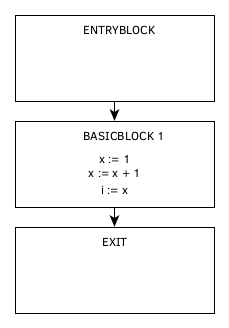
\includegraphics[width=0.3\textwidth]{assignments-only-cfg}
	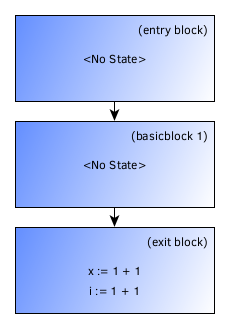
\includegraphics[width=0.3\textwidth]{assignments-only}
	\caption{Demonstration of simple assignments and reassignments. The resulting state is displayed on the next block.}
	\label{fig:assignmentOnly}
\end{figure}

\begin{figure}
	\begin{GenericCode}
if $x$ = 2 then 
	y $\leftarrow$ true
else
	y $\leftarrow$ false
end\end{GenericCode}
	\centering
	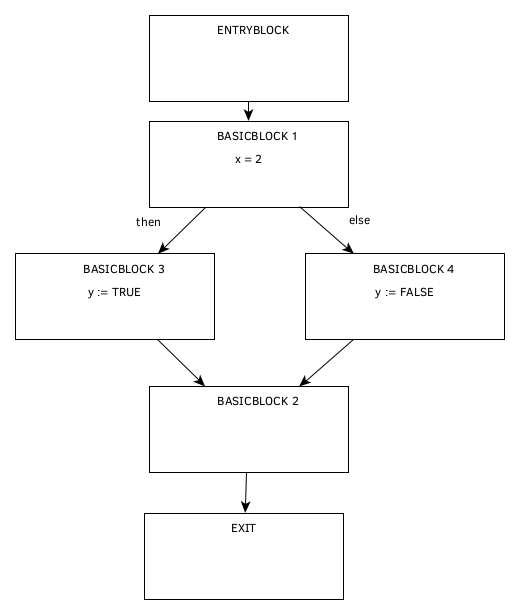
\includegraphics[width=0.4\textwidth]{simple-if-cfg}
	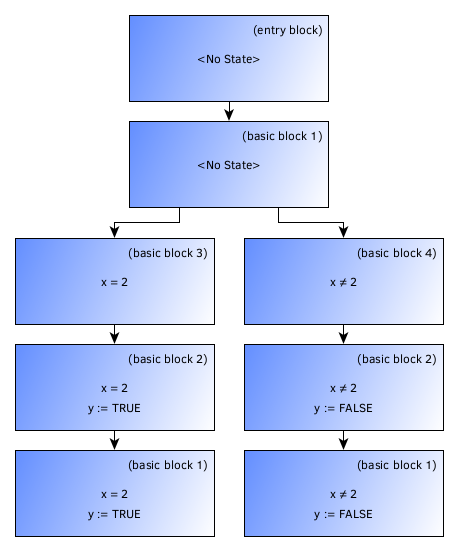
\includegraphics[width=0.4\textwidth]{simple-if}
	\caption{Simple selection (IF). The flow is divided into to branches - the condition could either be TRUE or FALSE. Each path will be evaluated separately. }
	\label{fig:simpleIf}	
\end{figure}

\begin{figure}
	\begin{GenericCode}
for $i$ $\leftarrow$ 0..$x$ do
	$y$ $\leftarrow$ $i$ + $x$
end	\end{GenericCode}
	\centering
	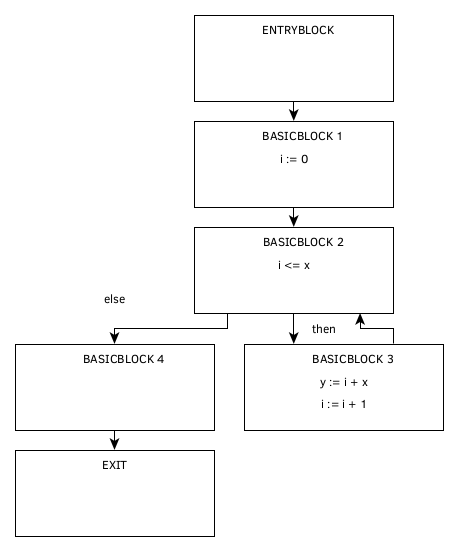
\includegraphics[width=0.4\textwidth]{simple-loop-cfg}
	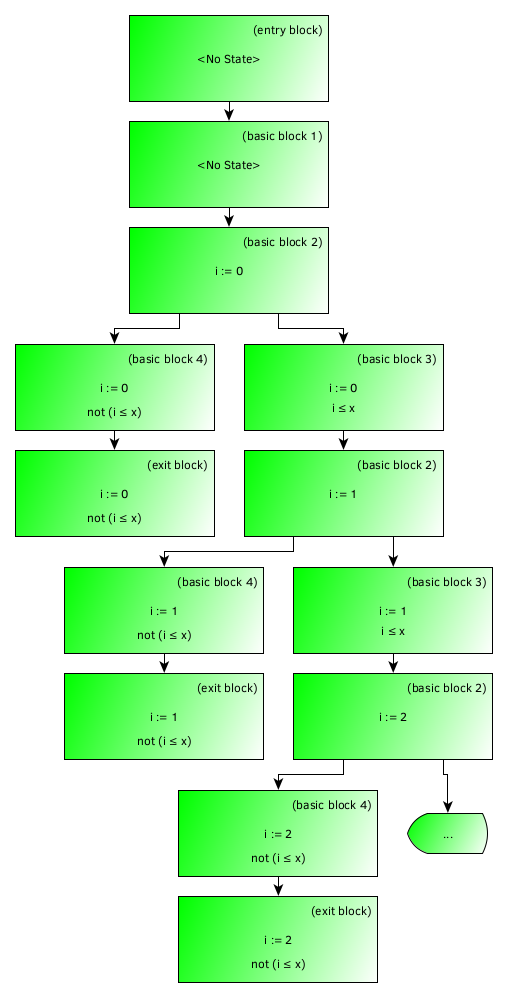
\includegraphics[width=0.4\textwidth]{simple-loop}
	\caption{After each iteration the condition will be evaluated with the new state again. Every node is reachable, even tough the analysis stopped prematurely, since the analysis could eventually be indefinitely. }
	\label{fig:simpleLoop}
\end{figure}

\begin{figure}
	\begin{GenericCode}
$i$ $\leftarrow$ 1
while $i$ < 10 do
	$i$ $\leftarrow$ 2
	break
	$i$ $\leftarrow$ 3
end\end{GenericCode}
	\centering
	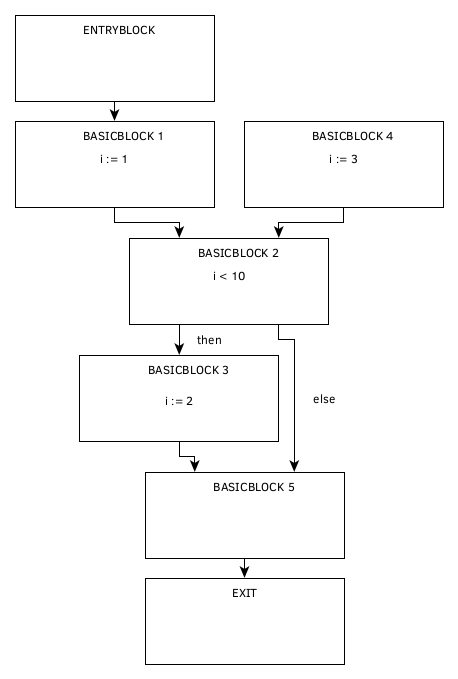
\includegraphics[width=0.4\textwidth]{unconditional-jump-cfg}
	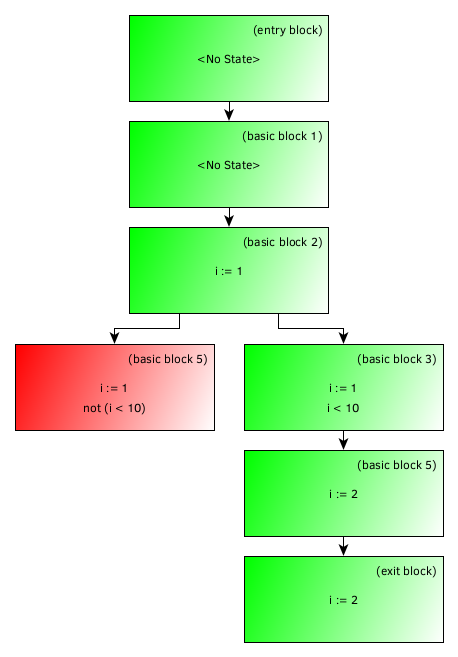
\includegraphics[width=0.4\textwidth]{unconditional-jump}
	\caption{Instruction block 4 is not reachable, since the flow was interrupted by an unconditional jump.}
	\label{fig:unconditionalJump}
\end{figure}

\subsection{Early stopping}
\label{sub:early stopping}
Ideally, there is an infinite amount of time available for the analysis. Realistically this is impossible to accomplish, therefore mechanisms to stop the computation early must be implemented.
Due to possible mutable state it is not easy to determine values without interpreting the flow of the program. 
% This is the main reason the approach \ref{cha:state of the art} does not detect possible unreachable Code in loops \ref{code:ssa-defect}. 
But being able to find this kind of defects comes with greater execution time. Without proper guards the analysis would take an infinite amount of resources and never find a solution.
\begin{itemize}
	\item One of the simplest mechanisms could be, that as soon as every instruction block is marked as reachable, the analysis should stop.
	\item As soon as loops are involved a multitude of different strategies would come to mind. 
	\begin{itemize}
		\item Following the flow of a loop a maximum set amount of time. Note that this approach could lead to false-positives, since the loop only finished partly. 
		\item Stopping the analysis as soon as too many iterations were made. No false positives will be reported, but the analysis is incomplete.
		\item Resetting the state of every assigned variable inside the body of the loop. Therefore no false positives will be reported, but may overlook some instances of unreachable code.
	\end{itemize}
\end{itemize}

\subsection{Handling Procedure - and Function-calls}
\label{sub:handling procedure and function calls}
Procedure and function calls are handled intraprocedurally, meaning return values are not calculated. That simply means every function call just checks if the declaration contains any (mutable) in and out parameters or is used on the right hand side of an assignment.
Either way said variables must reset their state, since the value may change. 
This approach is definitely lighter on resources (in contrast to interprocedural analysis), but may not be able to detect certain defects which may be obvious to a human. Consider the usage of the identity function. Since the intraprocedural approach does not consider the body of the called function, the state must reset the assigned variable, even tough it does not change.

\subsection{Problems and Barriers}
\label{sub:problems and barriers}
Especially the evaluation of loops is not gentle on resources and processing power. The number of blocks to evaluate grows exponentially. Naturally loops are very common. In theory this approach could find every instance of unreachable code, only limited by available resources. Multiple strategies described before in Section \ref{sub:early stopping} may be applied to reduce the number of iterations.
The consequences of these strategies are, that not every instance of unreachable code can be detected, making this method not necessarily superior to the traditionally implemented approach.
It may be possible to use some sort of preprocessing and potentially make it possible to evaluate loops only once, which could reduce the execution time drastically.
The implementation of such a form of preprocssing must take mutations into account and ideally guarantee the same accuracy.
Without any preprocessing interprocedural analysis of function-/procedure calls may also increase execution time significantly, since they must be interpreted as well. Here also some sort of preprocessing would be interesting. 
Recursive functions (directly and indirectly) would also lead to an increase of execution time.

%!TEX root = ../main.tex

\chapter {Evaluation}
\label {cha:evaluation}
This chapter contains interesting IEC functions and procedures, either found in production code or collected and translated from literature.
Each example provides the code, the control flow graph, a description and some metrics, like execution time, number of instruction blocks needed to conclude the result and, most importantly, the reported violations.


\section{Basic Example}
This example in Figure \ref{code:basic example 1 cfg} was found in production code and motivation for this implementation and thesis. There are no loops or procedure calls present, which change the variables provided as parameters (even though there are procedure calls, they cannot change them, since they are only declared as input variables).
Basically, this algorithm contains simple assignments and conditions, which eventually lead to unreachable code when combined, only.
As described at Figure \ref{code:basic example 1}, basic block 11 is not reachable, a consequence of the condition in line 15.
Even though a simple example on how unreachable code may look like in production code, it is easily demonstrated how code becomes unreachable by conditions, when they are combined.
The idea of the implementation originated from this example.

Metrics:
\begin{itemize}
	\item Runtime: 581 ms
	\item Number of analyzed instruction blocks: 17
	\item Violations: block 11
\end{itemize}

% 581ms
% 17 Blöcke analysiert
% Violation für block 11

\begin{figure}
	\begin{GenericCode}
IF s_operationHour <> m_operationHour THEN
	m_operationHour := s_operationHour;
	IF s_operationHour = 0 THEN
		RESET_ALARM(Name := er_service, SubID1 := m_iNumber);
	END_IF;
	RETURN;
END_IF;
// s_operationHour must be equal to m_operationHour
IF s_operationHour = 0 THEN
	// unnecessary - already zero
	m_operationHour := 0;
	RESET_ALARM(Name := er_service, SubID1 := m_iNumber);
ELSE
	// unreachable
	IF s_operationHour <> m_operationHour THEN
		s_operationHour := m_operationHour;
	END_IF;
END_IF;	\end{GenericCode}
	\centering

	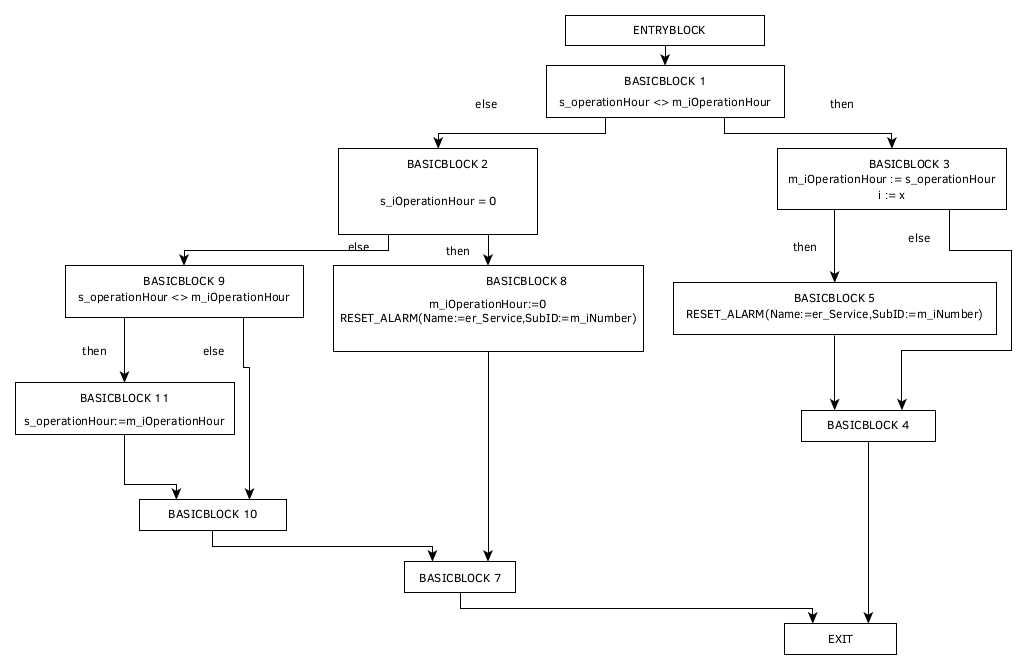
\includegraphics[width=0.9\textwidth]{minimal-example-cfg}
	\caption{A minimal example containing unreachable code due to unsatisfiable conditions. The condition in line 15 is never reachable, since this case was already handled in line 1 and the state of that variable did not change. Therefore basic block 11 is not reachable.}
	\label{code:basic example 1 cfg}
\end{figure}

\begin{figure}
	\centering
	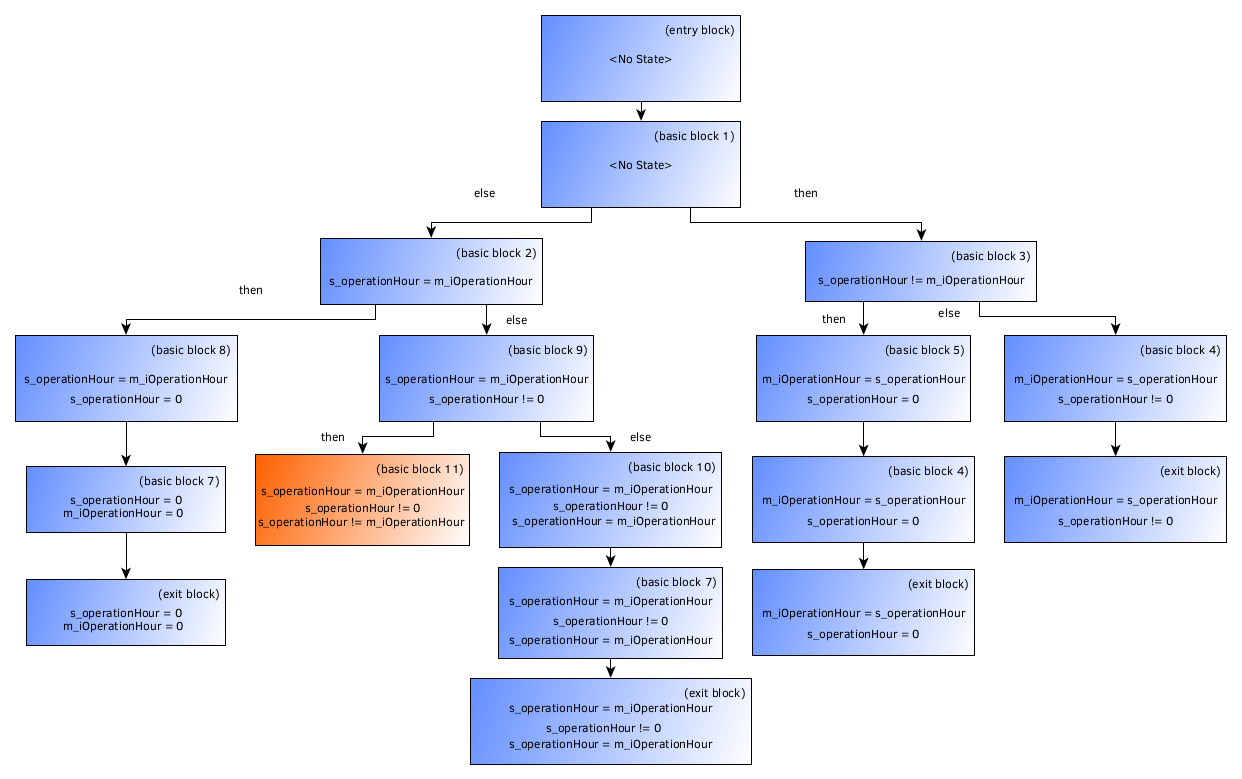
\includegraphics[width=1\textwidth]{minimal-example}
	\caption{Analysis of example \ref{code:basic example 1 cfg}. }
	\label{code:basic example 1}
\end{figure}

\section{Loops}
The main consequence of the implementation is significantly greater execution time, especially, when loops are present.
The following examples contain an almost identical algorithm. The only difference is that the first example in figure \ref{code:loop example 1 cfg} has a set value for x, whereas the example in figure \ref{code:loop example 2 cfg} does not have a limitation. Therefore basic block 6 is not reachable in the first example in figure \ref{code:loop example 1}, but may be reachable for the second example in figure \ref{code:loop example 2}.


Metrics (Example 1):
\begin{itemize}
	\item Runtime: 61 ms
	\item Number of analyzed instruction blocks: 20
	\item Violations: block 6
\end{itemize}



Metrics (Example 2):
\begin{itemize}
	\item Runtime: <1 ms
	\item Number of analyzed instruction blocks: 68
	\item Violations: none
\end{itemize}


\begin{figure}
	\begin{GenericCode}
i := 1;
x := 5;
		
WHILE i < x DO
	i := i + 1;
END_WHILE;
		
IF i = 3 THEN
	x := 4;
END_IF;	\end{GenericCode}
	\centering
	% 61ms
	% 20
	% Violation für block 6
	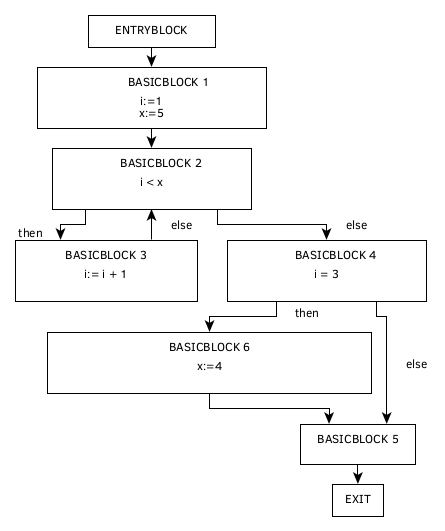
\includegraphics[width=0.6\textwidth]{basic-while-cfg}
	\caption{The variable i will change inside the loop. As long as x is not equal to 3, the basic block 6 is unreachable. }
	\label{code:loop example 1 cfg}
\end{figure}
\begin{figure}
	\centering
	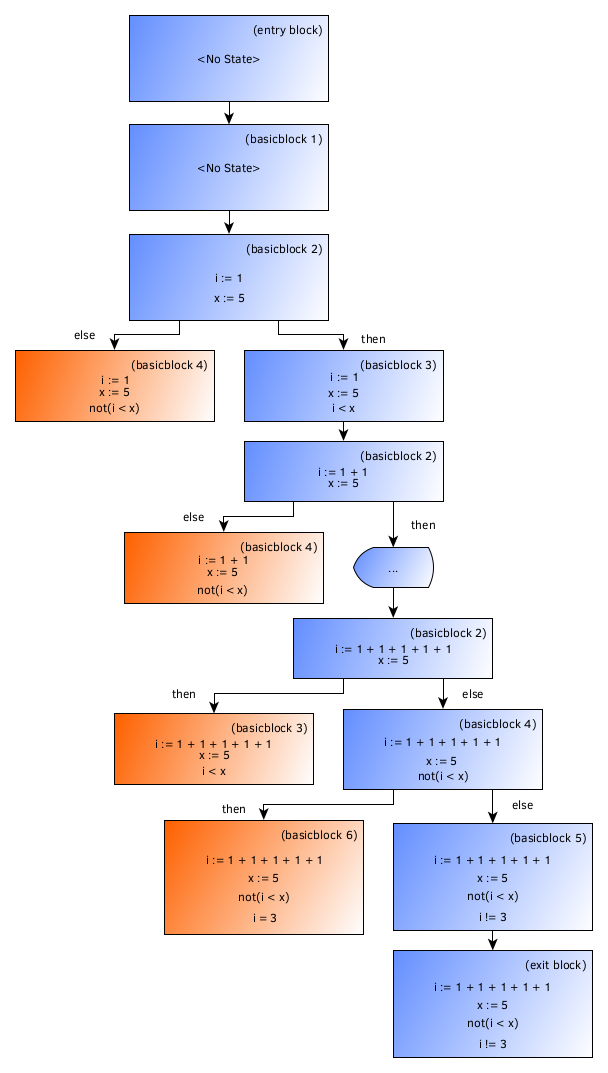
\includegraphics[width=0.6\textwidth]{basic-while}
	\caption{Analysis of example \ref{code:loop example 1 cfg}. }
	\label{code:loop example 1}
\end{figure}
\begin{figure}
	\begin{GenericCode}
i := 1;
		
WHILE i < x DO
	i := i + 1;
END_WHILE;
		
IF i = 3 THEN
	x := 4;
END_IF;		\end{GenericCode}
	\centering
	% <1ms
	% 68
	% No violations
	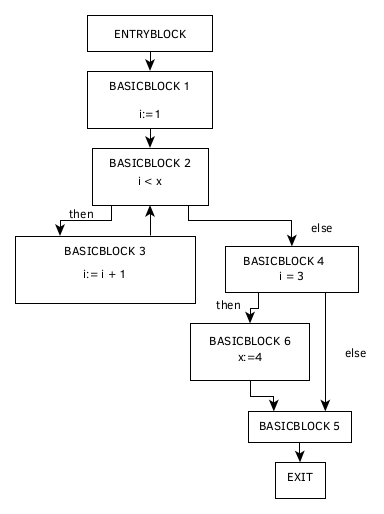
\includegraphics[width=0.6\textwidth]{basic-while-input-cfg}
	\caption{Same as \ref{code:loop example 1}, but x is an input variable. Therefore it may be 3, so it could be reachable.}
	\label{code:loop example 2 cfg}
\end{figure}
\begin{figure}
	\centering
	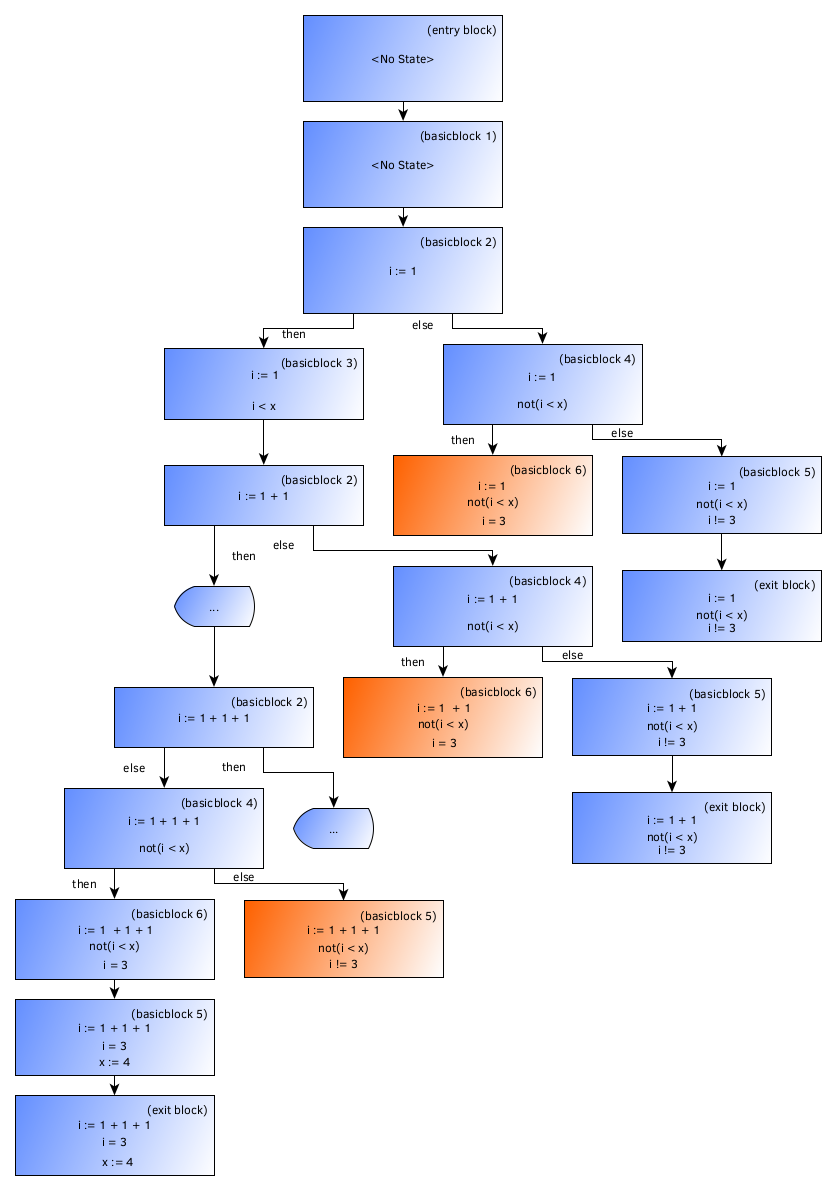
\includegraphics[width=0.8\textwidth]{basic-while-input}
	\caption{Analysis of example \ref{code:loop example 2 cfg}.}
	\label{code:loop example 2}
\end{figure}
\section{Function- and Procedure-Calls}
This example in Listing \ref{code:func test 1} demonstrates the handling of function- and procedure calls. It contains 2 different procedures: FooOutput and algo1 (which is part of an instantiated algorithm block). 
As described in Section, \ref{sub:handling procedure and function calls} only the declaration of parameters matters. Even if the function does not actually change the variable, it will be handled as such. 
Due to these circumstances, basic blocks 5 and 9 are not reachable.


Metrics:
\begin{itemize}
	\item Runtime: 169 ms
	\item Number of analyzed instruction blocks: 31
	\item Violations: block 5
\end{itemize}


\begin{program}
	\begin{GenericCode}
tmp1 := 1;
tmp2 := 2;
tmp3 := 3;

FooOutput(tmp1, tmp2, tmp3);

IF tmp2 <> 2 AND tmp3 <> 3 THEN
	tmp2 := 2; // Reachable - could change
END_IF;

IF tmp1 <> 1 THEN
	tmp2 := 3; // Unreachable
END_IF;

ABFunc.algo1(tmp2, tmp1, tmp3);

IF tmp1 <> 1 AND tmp3 <> 1 THEN
	tmp2 := 3; // Reachable
END_IF;

ABFunc.algo1(out1 => tmp1, in1 := tmp2, in_out1 := tmp3);

IF tmp2 = 3 THEN
	tmp2 := 3; // Reachable
END_IF;	\end{GenericCode}
	\centering
	% 169ms
	% 31 
	% Violations 5
	\caption{Demonstrates intraprocedural analysis. The procedure  FooOutput declares the first parameter as an IN parameter and therefore has no effect on the variable, while the other two parameters are declared as OUT parameters and might change. Note that the analysis does not check if the out parameter will be mutated, so it will be counted as if it would have. ABFunc is an instantiated algorithm block, which is similar to a class, and declares the parameters of the procedure \emph{algo1} in the same order. Note that the second occurrence of this method call contains named parameters. \emph{out1} and \emph{in\_out3} may be mutated.}
	\label{code:func test 1}
\end{program}
\begin{figure}
	\centering
	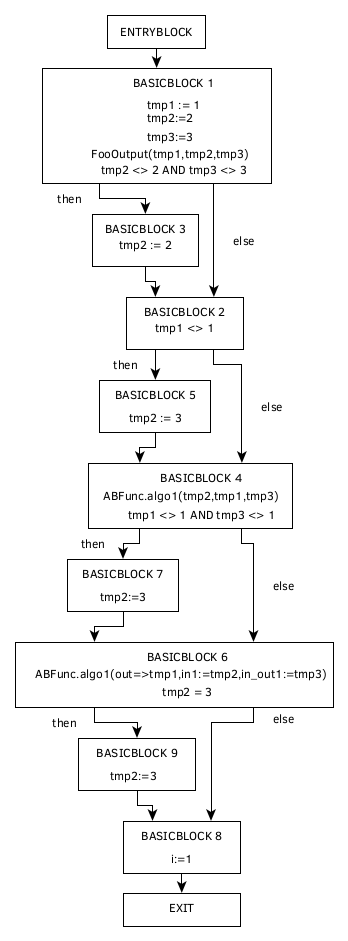
\includegraphics[width=0.5\textwidth]{easy-func-test-cfg}
	\caption{Control flow graph of example \ref{code:func test 1}}
	\label{fig:func test 1 cfg}
\end{figure}
\begin{figure}
	\centering
	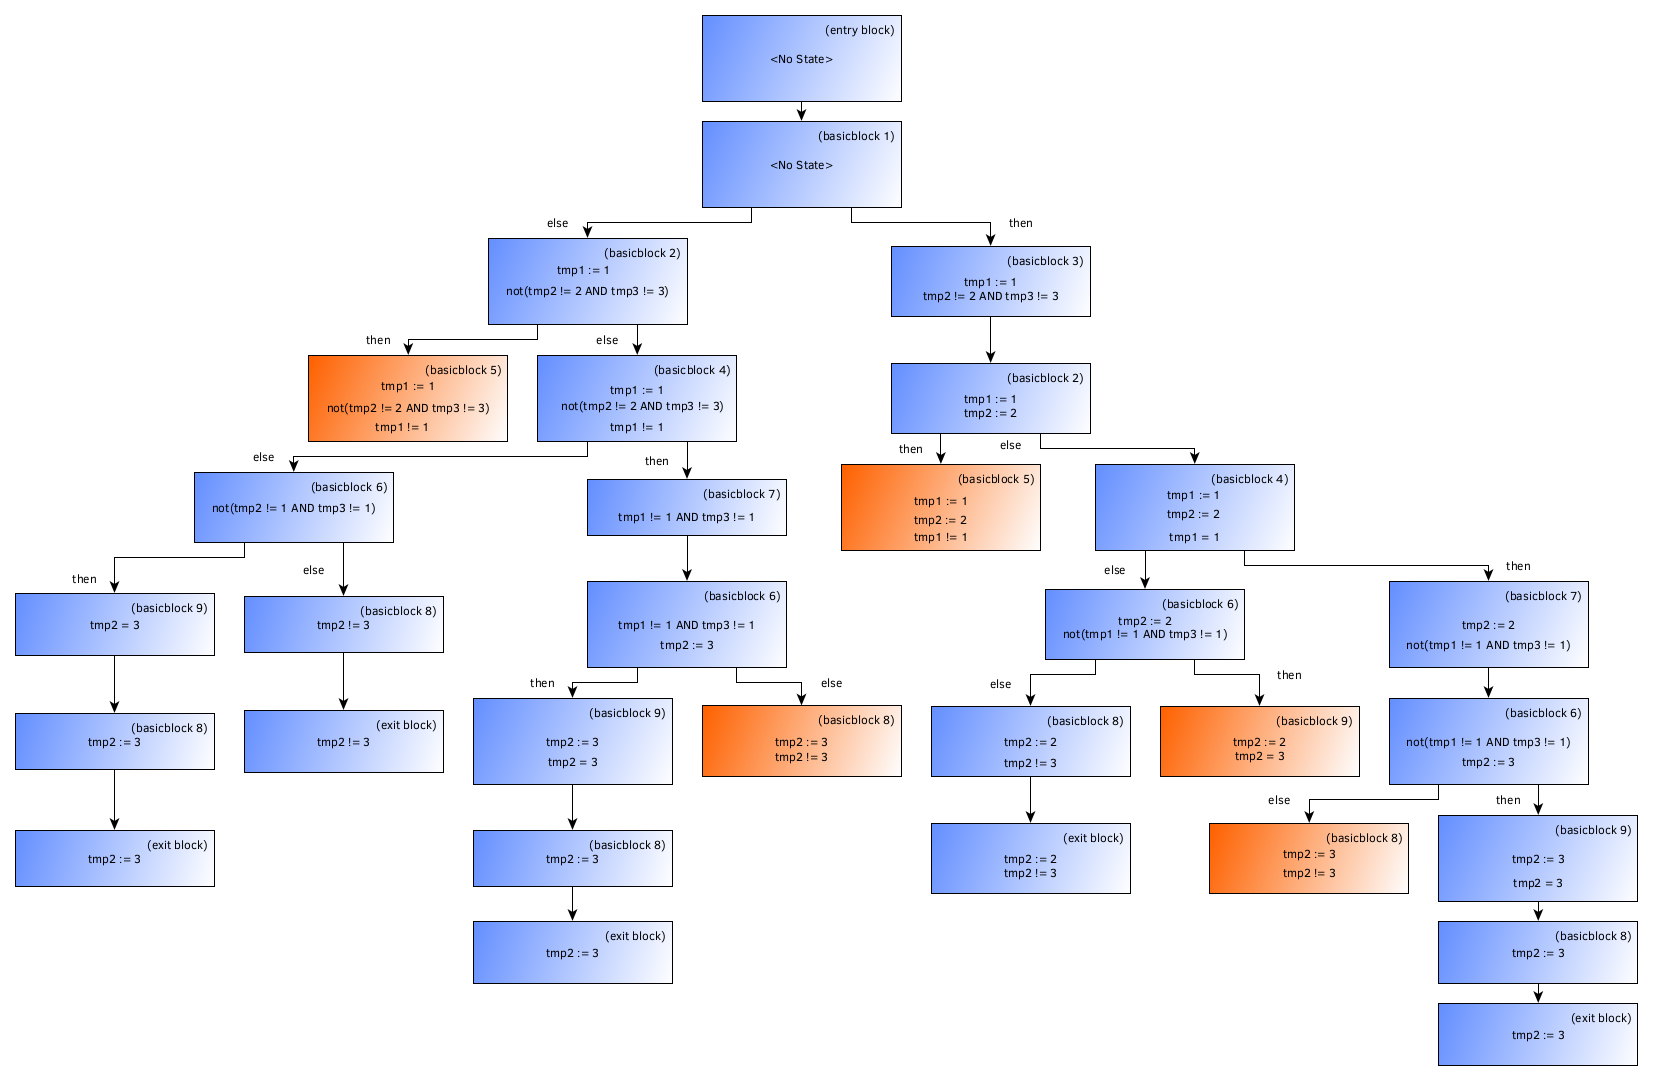
\includegraphics[width=1\textwidth]{easy-func-test}
	\caption{Analysis of example \ref{fig:func test 1 cfg}.}
	\label{fig:func test 1}
\end{figure}

\section{Hard Example}
This example in Figure \ref{code:hard example 1} and Figure \ref{code:hard example 1 cfg} was found in the literature \cite{Click_1995} and it was stated that the usual method for finding unreachable code is not able to detect this instance. 
Since the implementation is different at its core, it was only natural to test and compare the results.
Since no other functions were injected for this analysis, in contrast to the method described in chapter \ref{cha:state of the art}, this instance will be found and reported.
Note that the loop contains a variable which does not change, which will never stop. Therefore the analysis would stop early and no violation would be reported without the correct configuration. 
If the condition would have been different, it is easier to detect, but since this example has been used by different sources it was not altered.


Metrics:
\begin{itemize}
	\item Runtime: 20 ms
	\item Number of analyzed instruction blocks: 47
	\item Violations: block 4
\end{itemize}

\begin{figure}
	\begin{GenericCode}
x := 1;
	
REPEAT
	b := x <> 1;
	IF b = TRUE THEN
		x := 2;
	END_IF;    
UNTIL pred
END_REPEAT;	\end{GenericCode}
	% 20ms
	% 47
	% Violation Block 4
	\centering
	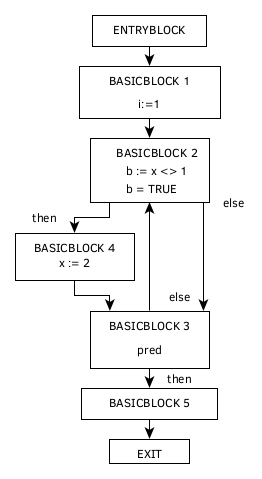
\includegraphics[width=0.4\textwidth]{hard-example-cfg}
	\caption{As described in \ref{code:ssa-defect} this procedure cannot be analyzed correctly and will not report that basic block 4 is unreachable. }
	\label{code:hard example 1}
\end{figure}
\begin{figure}
	\centering
	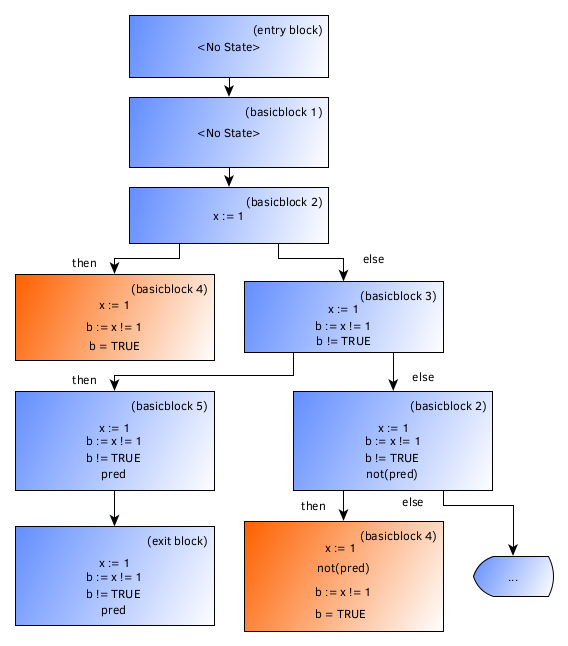
\includegraphics[width=0.7\textwidth]{hard-example}
	\caption{Analysis of example \ref{code:hard example 1 cfg}.}
	\label{code:hard example 1 cfg}
\end{figure}



%!TEX root = ../main.tex

\chapter{Conclusion}
\label{cha:conclusion}

The developed approach examines every possible path of a control flow graph and interprets all instructions, such as assignments, conditions and function/procedure calls for satisfiability. If a block can never be visited by the combination of previous assignments and conditions it is unreachable.

Even though procedures are checked intraprocedurally, rather than interprocedurally, the implementation provides good results. It is not only able to find basic instances of unreachable code, but also rather complicated incidents, which cannot be found by going for a traditional approach. 
The implementation could be the basis for other checks. SMT-solvers simplify checking predicates and the already existing architecture keeps the state of variables in check. 
Implementing different rules on top of that architecture may enable sophisticated checks, e.g., unnecessary code.
This possibility may be explored in the future.


As mentioned in Section \ref{sub:problems and barriers}, the downside of this approach is runtime. Programs containing loops, especially when nested, create many incidents that have to be checked. Since loops are one of the most essential instructions in programming, they occur often naturally. 
This complexity has to be addressed, because otherwise it does not make any sense to use this analysis in production, especially for bigger projects.


As demonstrated in Section \ref{code:hard example 1}, using correct configuration may be able to discover instances of unreachable code, which no other tool described in Chapter \ref{cha:state of the art} would be able to do. But this can only be done if the correct configuration is known, possibly leading to false positives. It is questionable if this approach is practicable.


Other tools, like sonarqube, as described in Section \ref{sec:sonar}, for example, do not offer to check loops to a full extent, but still manage to find a decent number of violations. Joogie, as described in Section \ref{sec:sca paper}, simplifies loops into three unwindings. Similar forms of preprocessing could reduce runtime significantly by trading a little bit of accuracy, making it usable in production environments. 




%%%----------------------------------------------------------
\appendix                                            % Anhang 
%%%----------------------------------------------------------

% \chapter{Technische Informationen}
\label{app:TechnischeInfos}

	% Technische Ergänzungen
% \chapter{Ergänzende Inhalte} % \chapter{Inhalt der CD-ROM/DVD}
\label{app:materials}


Auflistung der ergänzenden Materialien zu dieser Arbeit, die zur digitalen Archivierung an der 
Hochschule eingereicht wurden (als ZIP-Datei).

% Nur als Beispiel, die Struktur sollte man an die eigenen Bedürfnisse anpassen!

\section{PDF-Dateien}
\begin{FileList}{/}
\fitem{thesis.pdf} Finale Master-/Bachelorarbeit (Gesamtdokument)
\end{FileList}

\section{Mediendaten}
\begin{FileList}{/media}
\fitem{*.ai, *.pdf} Adobe Illustrator-Dateien
\fitem{*.jpg, *.png} Rasterbilder
\fitem{*.mp3} Audio-Dateien
\fitem{*.mp4} Video-Dateien
\end{FileList}


\section{Online-Quellen (PDF-Kopien)}
\begin{FileList}{/online-sources}
\fitem{Reliquienschrein-Wikipedia.pdf} \citenobr{WikiReliquienschrein2018}
\end{FileList}



	% Inhalt der CD-ROM/DVD
% \chapter{Fragebogen}
\label{app:Fragebogen}

	% Chronologische Liste der Änderungen
% \chapter{\latex-Quellcode}
\label{app:Quellcode}

	% Quelltext dieses Dokuments

%%%----------------------------------------------------------
\MakeBibliography % Quellenverzeichnis
%%%----------------------------------------------------------
%%% Messbox zur Druckkontrolle ------------------------------
\chapter*{Messbox zur Druckkontrolle}



\begin{center}
{\Large --- Druckgröße kontrollieren! ---}

\bigskip

\calibrationbox{100}{50} % Angabe der Breite/Hoehe in mm

\bigskip

{\Large --- Diese Seite nach dem Druck entfernen! ---}

\end{center}


%%%----------------------------------------------------------
\end{document}
%%%----------------------------------------------------------
